\documentclass{article}

% Important packages to use
\usepackage[utf8]{inputenc}
\usepackage{amssymb}
\usepackage{amsthm}
\usepackage{amsmath}
\usepackage{geometry}
\usepackage{graphicx}
\RequirePackage[12tabu, orthodox]{nag}
\usepackage{microtype} 	% impoves spacing
\usepackage{siunitx}	% simplify TeXing
\usepackage{cleveref}
\usepackage[colorlinks=false]{hyperref}

% Set line spacing in enumerate
\usepackage{enumitem}
\usepackage{lipsum}
\setlist[enumerate]{topsep=0pt,itemsep=-3ex,partopsep=1ex,parsep=1ex}

% Table of contents section
% -1 part     1 section     3 subsubsection  5 subparagraph
%  0 chapter  2 subsection  4 paragraph
\setcounter{tocdepth}{3}

% Automatic parenthesizing
% \usepackage{nath}
% \delimgrowth=1

% pseudocode
\usepackage{algorithmicx}
\usepackage{algpseudocode}

%%%%%%%%%%%%%%%%%%%%%%%%%%%%%%%%%%%%%%%%%%%%%%%%%%%%%%%%%%%%%
%%%%%%%%%%%%%%%%%%%%%%%%%%%%%%%%%%%%%%%%%%%%%%%%%%%%%%%%%%%%%
%%
%% TITLE
%%
%%%%%%%%%%%%%%%%%%%%%%%%%%%%%%%%%%%%%%%%%%%%%%%%%%%%%%%%%%%%%
%%%%%%%%%%%%%%%%%%%%%%%%%%%%%%%%%%%%%%%%%%%%%%%%%%%%%%%%%%%%%
\title{Machine Learning}
\author{Teerapat (Mek) Jenrungrot}
\date{ }

\begin{document}
\maketitle

\tableofcontents

\section{Supervised Learning}
\subsection{Part I: Linear Regression}
Let $\theta_i$'s be the {\bf parameters} (also called {\bf weights}) paramaterizing the space of linear functions mapping from $\mathbb{X}$ to $\mathbb{Y}$. We make the notation, with $x_0 = 1$,

\begin{equation}
	\label{eq:hypothesis_function}
	h(x) = \sum_{i=0}^{n}\theta_i x_i = \theta^Tx
\end{equation}
as a hypothesis $h$ where on the right-hand side above we are vieweing $\theta$ and $x$ both as vectors, and here $n$ is the number of input variables (not counting $x_0$).

We now define the {\bf cost function}:
\begin{equation}
	\label{eq:cost_function}
	J(\theta) = \frac{1}{2}\sum_{i=1}^{m}(h_\theta(x^{(i)}) - y^{(i)})^2.
\end{equation}

\subsubsection{LMS algorithm}
\paragraph{gradient descent} We consider the {\bf gradient descent} algorithm, which starts with some initial $\theta$, and repeatedly performs update:
\begin{equation}
	\theta_j := \theta_j - \alpha\frac{\partial}{\partial \theta_j}J(\theta).
\end{equation}
Here, $\alpha$ is called the {\bf learning rate}.
In order to implement this algorithm, we need to work out what is the partial derivative term on the right hand side. Let's first work it out for the case of if we have only one training example $(x,y)$, so that we can neglect the sum in the definition of $J$. We have:
\begin{align*}
	\frac{\partial}{\partial\theta_j}J(\theta) &= \frac{\partial}{\partial\theta_j}\frac{1}{2}(h_\theta(x)-y)^2 \\
	&= 2\cdot\frac{1}{2}(h_\theta(x)-y)\cdot\frac{\partial}{\partial\theta_j}(h_\theta(x)-y)\\
	&= (h_\theta(x)-y)\cdot\frac{\partial}{\partial\theta_j}\left(\sum_{i=0}^{n}\theta_ix_i-y\right) \\
	&= (h_\theta(x)-y)x_j
\end{align*}
Thus, for a single training example, this gives the update rule:
\begin{equation}
	\label{eq:update_rule}
	\theta_j := \theta_j + \alpha\left(y^{(i)}-h_\theta(x^{(i)})\right)x_j^{(i)}.
\end{equation}
\paragraph{batch gradient descent} This algorithm looks at every example in the entire training set on every step.
\begin{algorithmic}
\Repeat
	\State $\theta_j \gets \theta_j + \alpha \sum_{i=1}^{m}\left(y^{(i)} - h_\theta(x^{(i)})\right)x_j^{(i)}$
\Until{ it is convergence }
\end{algorithmic}
\paragraph{stochastic gradient descent} This algorithm updates the parameters according to the gradient of the error with respect to that single training example only.
\begin{algorithmic}
\Loop
	\For{$i = 1$ to $m$}
		\State $\theta_j \gets \theta_j + \alpha \left(y^{(i)} - h_\theta(x^{(i)})\right)x_j^{(i)}$
	\EndFor
\EndLoop
\end{algorithmic}

\subsection{The normal equations}
In this section, we will discuss a second way of minimizing $J$ by using derivatives.
\subsubsection{Matrix derivatives}
\paragraph{$\nabla_A f(A)$} For a function $f: \mathbb{R}^{m \times n} \rightarrow \mathbb{R}$, we define the derivative of $f$ with respect to $A$ to be:
\begin{equation}
	\label{eq:gradient_definition}
	\nabla_A f(A) =
	\begin{bmatrix}
		\frac{\partial f}{\partial A_{11}} & \ldots & \frac{\partial f}{\partial A_{1n}} \\
		\vdots & \ddots & \vdots \\
		\frac{\partial f}{\partial A_{m1}} & \ldots & \frac{\partial f}{\partial A_{mn}}
	\end{bmatrix}
\end{equation}
\paragraph{trace operation} We define the {\bf trace} operator as:
\begin{equation}
	\label{eq:trace_definition}
	\text{tr} A = \sum_{i=1}^{n}A_{ii}
\end{equation}
We'll now prove that $\text{tr} (AB) = \text{tr} (BA)$ if $AB$ is square:
\begin{align*}
	\text{tr} (AB) &= \sum_{i=1}^{n}(AB)_{ii} \\
	&= \sum_{i=1}^{n}\sum_{j=1}^{n}a_{ij}b_{ji} \\
	&= \sum_{j=1}^{n}\sum_{i=1}^{n}b_{ji}a_{ij} \\
	&= \sum_{j=1}^{n}(BA)_{jj} \\
	&= \text{tr} (BA)
\end{align*}
Followings are some more facts of matrix derivatives for if both $A$ and $B$ are square matrices:
\begin{align}
	\label{eq:gradient_equations}
	\nabla_A \text{tr} AB &= B^T \\
	\nabla_{A^T} f(A) &= \left(\nabla_A f(A)\right)^T \\
	\nabla_A \text{tr} ABA^TC &= CAB + C^TAB^T \\
	\nabla_A |A| &= |A| \left(A^{-1}\right)^T
\end{align}

\subsubsection{Least squares revisited}
\paragraph{design matrix} Given a training set, define the \textbf{design matrix} $X$ to be the $m$-by-$(n+1)$ matrix (including the intercept term) that contains the training examples' input values in its row:
\begin{equation}
	\label{eq:design_matrix}
	X =
	\begin{bmatrix}
		- \left(x^{(1)}\right)^T -\\
		- \left(x^{(2)}\right)^T -\\
		\vdots \\
		- \left(x^{(m)}\right)^T -\\
	\end{bmatrix}
\end{equation}
Let $\vec{y}$ be the $m$-dimensional vector containing all the target values from the training set:
\begin{equation}
	\label{eq:target_values}
	\vec{y} =
	\begin{bmatrix}
		y^{(1)} \\
		y^{(2)} \\
		\vdots \\
		y^{(m)}
	\end{bmatrix}
\end{equation}
Now, since $h_\theta\left(x^{(i)}\right)^T\theta$, we can easily verify that
\begin{align*}
	X\theta - \vec{y} &=
	\begin{bmatrix}
		\left(x^{(1)}\right)^T\theta \\
		\left(x^{(2)}\right)^T\theta \\
		\vdots \\
		\left(x^{(m)}\right)^T\theta \\
	\end{bmatrix}
	-
	\begin{bmatrix}
		y^{(1)} \\
		y^{(2)} \\
		\vdots \\
		y^{(m)}
	\end{bmatrix} \\
	&=
	\begin{bmatrix}
		h_\theta\left(x^{(1)}\right) - y^{(1)} \\
		h_\theta\left(x^{(2)}\right) - y^{(2)} \\
		\vdots \\
		h_\theta\left(x^{(m)}\right) - y^{(m)} \\
	\end{bmatrix}.
\end{align*}
Thus, using the fact that for a vector $z$, we have that $z^Tz = \sum_{i}z_i^2$:
\begin{align*}
	\frac{1}{2}\left(X\theta - \vec{y}\right)^T\left(X\theta - \vec{y}\right) &= \frac{1}{2} \sum_{i=1}^{m}\left(h_\theta(x^{(i)}) - y^{(i)}\right)^2 \\
	&= J(\theta)
\end{align*}
Finally, to minimize $J$, we find its derivative with respect to $\theta$:
\begin{align*}
	\nabla_\theta J(\theta) &= \nabla_\theta \frac{1}{2}\left(X\theta - \vec{y}\right)^T\left(X\theta - \vec{y}\right) \\
	&= \frac{1}{2} \nabla_\theta \left( \theta^TX^TX\theta - \theta^TX^T\vec{y} - \vec{y}^TX\theta + \vec{y}^T\vec{y} \right) \\
	&= \frac{1}{2} \nabla_\theta \text{tr} \left( \theta^TX^TX\theta - \theta^TX^T\vec{y} - \vec{y}^TX\theta + \vec{y}^T\vec{y} \right) \\
	&= \frac{1}{2} \nabla_\theta \left( \text{tr} \theta^TX^TX\theta -2\text{tr}\vec{y}\right) \\
	&= \frac{1}{2} \left(X^TX\theta + X^TX\theta - 2X^T\vec{y}\right) \\
	&= X^TX\theta - X^T\vec{y}
\end{align*}
To minimize $J$, we set its derivative to zero, and obtain the {\bf normal equations}:
\begin{equation}
	\label{eq:normal_equation}
	X^TX\theta = X^T\vec{y}
\end{equation}
Thus, the value of $\theta$ that minimizes $J(\theta)$ is given in closed form by the equation
\begin{equation}
	\theta = (X^TX)^{-1}X^T\vec{y}.
\end{equation}

\section{Statistical Learning}
\subsection{Measuring the Quantity fit}

\paragraph{Mean squared error}
The book defines the \textit{mean squared error} (MSE), given by
\[
	MSE = \frac{1}{n}\sum_{i=1}^{n}\left(y_i - \hat{f}(x_i)\right)^2
\]
where $\hat{f}(x_i)$ is the prediction that $\hat{f}$ gives for the $i$th observation. This value will be small if the predicted responses are very close to the true responses. Otherwise, the predicted value will be sunstantially high due to possibly bad predictors.

\paragraph{degree of freedom}
In short, \textbf{degree of freedom} describes the flexibility of a curve. The higher value of degree of freedom results in a highly fluctuating curve.

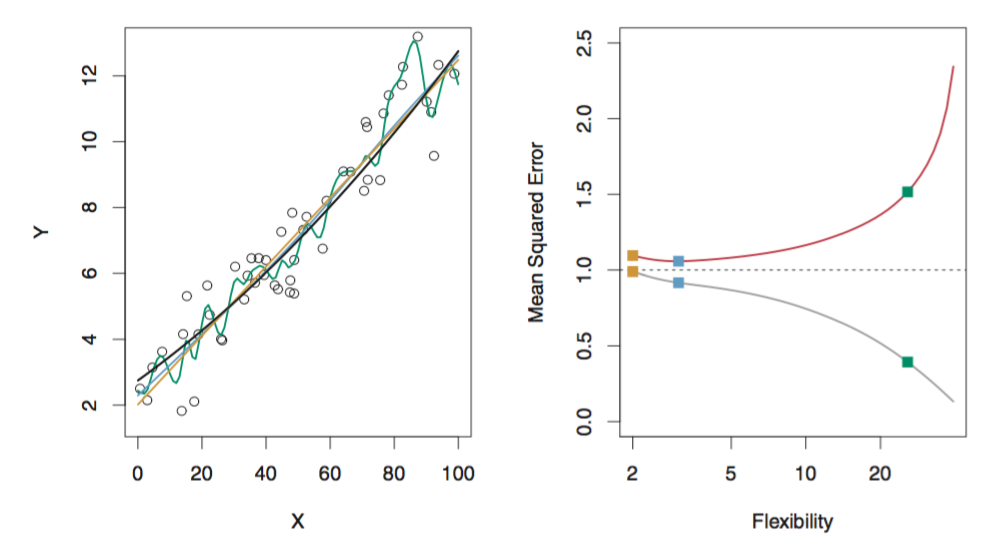
\includegraphics[scale=0.8]{images/flexibility_vs_mse.png} \\
This graph shows an example that the true $f$ is approximately linear. We observe that the training MSE decreases monotonically as the model flexibility increases, and that there is a U-shape in the test MSE. However, because the truth is so close to linear, the test MSE only decreases slightly before increasing again, so that \textbf{the orange least squares fit is substantially better than the highly flexible green curve}.

\subsection{The Bias-Variance Trade-Off}
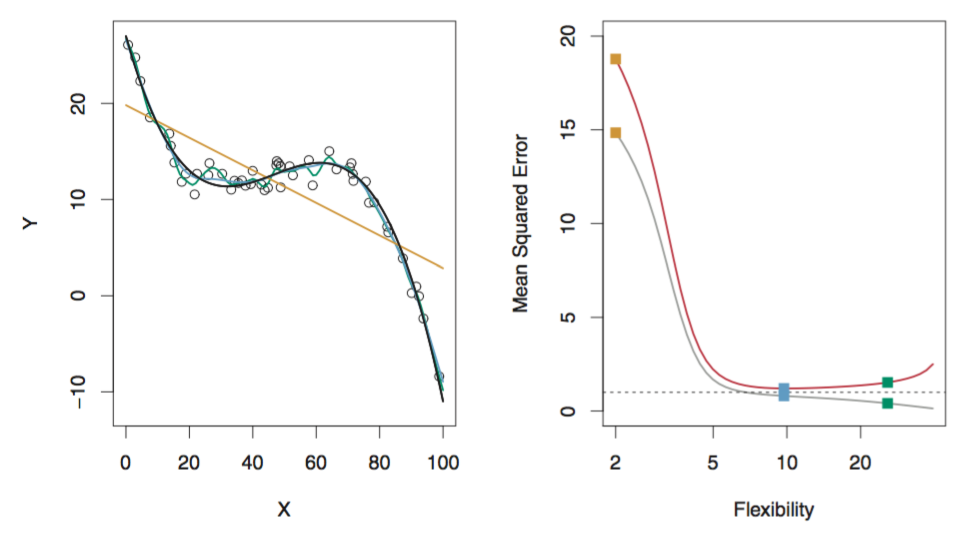
\includegraphics[scale=0.8]{images/linear_poorly_fits.png} \\
This graphs shows an example that the linear least square fit (as shown in the orange line) poorly fits the true $f$.

\paragraph{Expected test MSE} It is possible to show that the \textbf{expected test MSE}, for a given value $x_0$, can always be decomposed into the sum of three fundamental quantities: the \textit{variance} of $\hat{f}(x_0)$, the squared \textit{bias} of $\hat{f}(x_0)$, and the variance of the error terms $\epsilon$. That is,
\[
	E\left(y_0 - \hat{f}(x_0)\right)^2 = \text{Var}(\hat{f}(x_0)) + \left[\text{Bias}(\hat{f}(x_0))\right]^2 + \text{Var}(\epsilon).
\]
We need to select a statistical learning method that simulataneously achieves low variance and low bias.

\paragraph{Variance} Variance in this context refers to the amount by which $\hat{f}$ would change if we estimated it using a different training set. Since the training data are used to fir the statistical learning method, different training data sets will result in a different $\hat{f}$. But ideally the estimate for $f$ should not vary too much between training sets. However, if a method has high variance then small changes in the training data can result in large changes in $\hat{f}$. In general, more flexible statistical methods have higher variance.

\paragraph{bias} On the other hand, \textit{bias} refers to the error that is introduced by approximating a real-life problem, which may be extremely complicated, by a much simpler model. For example, linear regression assumes that there is a linear relationship between $Y$ and $X_1, X_2, \ldots, X_p$. It is unlikely that any real-life problem truly has such a simple linear relationship, and so performing linear regression will undoubted result in some bias in the estimate of $f$. \textbf{As a general rule, as we use more flexible methods, the variance will increase and the bias will decrease}.

\subsection{The Classification Setting}
\paragraph{the training error rate} We define it as
\[
	\frac{1}{n}\sum_{i=1}^{n}I(y_1 \ne \hat{y}_i).
\]
Here $\hat{y}_i$ is the predicted class label for the $i$th observation using $\hat{f}$. And $I(y_i \ne \hat{y}_i)$ is an indicator variable that equals 1 if $y_i \ne \hat{y}_i$ and 0 otherwise. A good classifier is one for which the test error is smallest.

\paragraph{The Bayes Classifier}
We classify data by assigning them to their most likely class, given thier predictor values. In other words, we should simple assign a test observation with predictor vector $x_0$ to the class $j$ for which
\[
	\text{Pr}(Y = j | X = x_0)
\]
is largest. To illustrate, in a two-class problem, the Bayes classifier corresponds to predicting class one if $\text{Pr}(Y = 1 | X = x_0) > 0.5$, and class two otherwise.

\paragraph{K-Nearest Neighbors}
In theory we would always like to predict qualitative responses using the Bayes classifier. But for real data, we do not know the conditional distribution of $Y$ given $X$, and so computing the Bayes classifier is impossible. K-nearest neighbors (KNN) classifier can solve such a problem. Given a positive integer $K$ and a test observation $x_0$, the KNN classifier first identifies the $K$ points in the training data that are closest to $x_0$, represented by $N_0$. It then estimates the conditional probability for class $j$ as the fraction of points in $N_0$ whose response values equal $j$:
\[
	Pr(Y = j | X = x_0) = \frac{1}{K}\sum_{i\in N_0}I(y_i = j).
\]
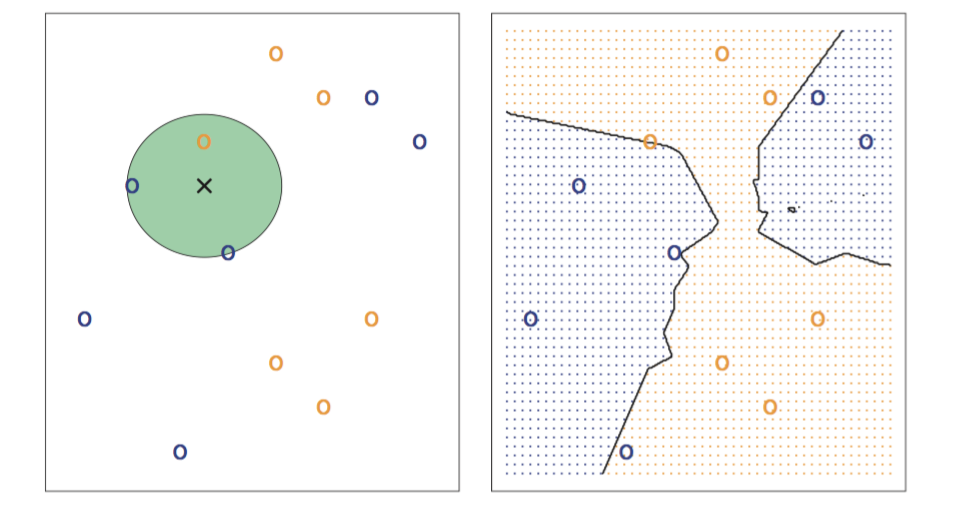
\includegraphics[scale=0.8]{images/knn1.png} \\

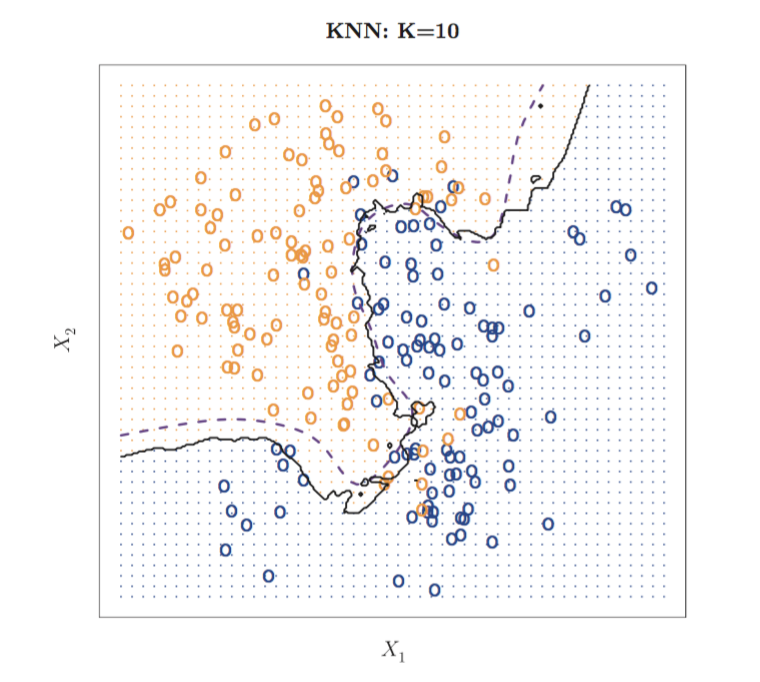
\includegraphics[scale=0.8]{images/knn2.png} \\
These images show the examples of KNN classifier.



\section{Classification}
Ref. ISLR Book
Examples:
\begin{enumerate}
\item A person arrives at the emergency room with a set of symptoms that could possibly be attributed to one of three medical conditions. Which of the three conditions does the individual have?
\item An online banking service must be able to determine whether or not a transaction being performed on the site is fraudulent, on the basis of the user's IP address, past transaction history, and so forth.
\item On the basis of DNA sequence data or a number of patients with and without a given disease, a biologist would like to figure out which DNA mutations are deleterious (disease-causing) and which are not.
\end{enumerate}

\subsection{Why Not Linear Regression?}
Suppose that we are trying to predict the medical condition of a patient in the emergency room on the basis of her symptoms. In this simplified example, there are three possible diagnoses. Least square could be used to fit a linear regression model to predict $Y$ on the basis of a set of predictors $X_1, \ldots, X_p$.

By doing so, the problem occurs because the order of three possible outcomes matter, e.g. the question arises if the first outcome should be between other two. This implies a different relationship among the three conditions. Each of these different orders can produce fundamentally different linear models that would ultimately lead to different sets of predictions on test observations.

For a binary qualitative response, the situation is better. However, for linear regression, some of our estimates might be outside the $[0,1]$ interval, making them hard to interpret as probabilities. Nevertheless, the predictions provide an ordering and can be interpreted as crude probability estimates.

\subsection{Logistic Regression}
The problem from using linear regression gives rise to the logistic model. We introduce a model:
\[
	p(X) = \frac{e^{\beta_0 + \beta_1X}}{1 + e^{\beta_0 + \beta_1X}}
\]
which the output of the function is in the interval $[0,1]$ for all values of $X$.

To fit the model above, we use a method called \textit{maximum likelihood}, which we will discuss in the next subsection. The logistic function will always produce an \textit{S-shaped} curve of this form, and so regardless of the value of $X$, we will obtain a sensible prediction.

After a bit of manipulation of the equation above, we find that
\[
	\frac{p(X)}{1-p(X)} = e^{\beta_0 + \beta_1X}
\]
\[
	\log\left(\frac{p(X)}{1-p(X)}\right) = \beta_0 + \beta_1X
\]
which shows that the logistic regression model has a logit that is linear in $X$.

\subsection{Estimating the Regression Coefficients}
Even though we can use the least squares approach to estimate the unknown linear regression coefficients above, the more general method of \textit{maximum likelihood} is preferred, since it has better statistical properties.

The basic intuition behind using maximum likelihood to fit a logistic regression model is as follows: we seek estimates for $\beta_0$ and $\beta_1$ such that the predicted probability $\hat{p}(x_i)$ of default for each individual, using the logistic model, corresponds as closely as possible to the individual's observed default status. In other words, we try to find $\hat{\beta}_0$ and $\hat{\beta}_1$ such that plugging these estimates into the model for $p(X)$ yield s a number close to one for all individuals who defaulted, and a number close to zero for all individual who did not. This intuition can be formalized using a mathematical equation called a \textit{likelihood function}:
\[
	l(\beta_0,\beta_1) = \prod_{i:y_i=1}p(x_i) \cdot \prod_{i':y_{i'}=0}(1-p(x_{i'}))
\]
The estimates $\hat{\beta}_0$ and $\hat{\beta}_1$ will be chosed to maximuze this likelihood function.

\subsection{Linear Discriminant Analysis}
Logistic regression involves directly modeling $\Pr(Y=k | X= x)$ using the logistic function. We now consider an alternative approach to estimatating these probabilities, which we model the distribution of the predictors $X$ separately in each of the response classes $Y$, and then use Bayes' theorem to flip these around into estimates for $\Pr(Y = k| X = x)$. Here are several reasons of doing so:
\begin{enumerate}
\item When the classes are well-separated, the paramater estimates for the logistic regression model are surprisingly unstable. Linear discriminant analysis does not suffer from this problem. \\
\item If $n$ is small and the distribution of the predictors $X$ is approximately normal in each of the classes, the linear discriminant model is again more stable than the logistic regression model. \\
\item Linear discriminant analysis is popular when we have more than two response classes.
\end{enumerate}

\subsubsection{Using Bayes' Theorem for Classification}
The Bayes' Theorem states that
\[
	\Pr(Y = k|X = x) = \frac{\pi_k f_k(x)}{\sum_{i=1}^{K}\pi_i f_i(x)}
\]
\subsubsection{Linear Discriminant Analysis for p = 1}
For now, we assume that $p = 1$, that is, we have only one predictor. We would like to obtain an estimate for $f_k(x)$ in order to estimate $p_k(x)$. We will then classify an observation to the class for which $p_k(x)$ is greatest. \\ \\

In order to estimate $f_k(x)$, we make some assumptions about its form. We assume that $f_k(x)$ is normal or Gaussian. In the one-dimensional setting, the normal density takes the form
\[
	f_k(x) = \frac{1}{\sqrt{2\pi}\sigma_k}\exp\left(-\frac{1}{2\sigma_k^2}(x - \mu_k)^2\right)
\]
where $\mu_k$ and $\sigma_k^2$ are the mean and variance parameters for the $k$th class. For now, let further assume that $\sigma_1^2 = \ldots = \sigma_K^2$: that is, there is a shared variance term across all $K$ classes, which for simplicity we can denote by $\sigma^2$. We then find that
\[
	p_k(x) = \frac{\pi_k \frac{1}{\sqrt{2\pi}\sigma}\exp\left(-\frac{1}{2\sigma^2}(x - \mu_k)^2\right)}{\sum_{l=1}^{K}\pi_l\frac{1}{\sqrt{2\pi}\sigma}\exp\left(-\frac{1}{2\sigma^2}(x - \mu_l)^2\right)}
\]
Note that $\pi_k$ denotes the prior probability than an observation belongs to the $k$th class.

To be added.

\subsubsection{Linear Discriminant Analysis for p > 1}
\subsubsection{Quadratic Discriminant Analysis}


\section{Implementation - Python}
\subsection{Classification}
\subsubsection{Machine Learning Basics}
The steps in developing a machine learning application:
\begin{enumerate}
	\item Collect data. \\
	\item Prepare the input data. \\
	\item Analyze the input data. \\
	\item Make sure the data don't have garbage coming in. \\
	\item Train the algorithm. \\
	\item Test the algorithm. \\
	\item Use it. \\
\end{enumerate}
We decide to use Python because of its clear syntax and extremely easy text manipulation. A large number of people around the world are using Python, so there are abundant development and documentation about machine learning.

We will also focus on using NumPy library for doing some linear algebra. For NumPy, there are two different data types for dealing with rows and columns of numbers. Be careful of this because they look similar, but simple mathematical operations such as multiply on the two data types can have different meanings. The matrix data type behaves more like matrices in MATLAB.
\subsubsection{Classification with k-Nearest Neighbors}

\textbf{k-Nearest Neighbors} \\
Pros: High accuracy, insensitive to outliers, no assumptions about data \\
Cons: Computationally expensive, requires a lot of memory \\
Works with: Numeric values, nominal values \\

\textbf{General approach to kNN} \\
\begin{enumerate}
	\item Collect: Any method. \\
	\item Prepare: Numeric values are needed for a distance calculation. A structured data format is best. \\
	\item Analyze: Any method. \\
	\item Train: Does not apply to the kNN algorithm. \\
	\item Test: Calculate the error rate. \\
	\item Use: This application needs to get some input data and output structured numeric values. Next, the application runs the kNN algorithm on this input data and determines which class the input data should belong to. The application then takes some action on the calculated class.
\end{enumerate}

\paragraph{Prepare: Importing data with Python}


\section{Image Classification (CS231n)}
\paragraph{Motivation} This is one of the core problems in Computer Vision that, despite its simplicity, has a very large variety of practical applications. Moreover, as we will see later in the course, many other seemingly distinct Computer Vision tasks (such as object detection, segmentation) can be reduced to image classification.

\paragraph{Example} You want to create a classification model that takes a single image and assigns probabilities to 4 labels, {cat, dog, hat, mug}. An image is represented as one large 3-dimensional array of numbers (Width x Height x RGB). Each number is an integer that ranges from 0 (black) to 255 (white).

\paragraph{Challenges}
The following challenges are worth considered:
\begin{enumerate}
	\item \textbf{Viewpoint variation}: A single instance of an object can be oriented in many ways with respect to the camera. \\
	\item \textbf{Scale Variation}: Visual classes often exhibit variation in their size.\\
	\item \textbf{Deformation}: Many objects of interest are not rigid bodies and can be deformed in extreme ways. \\
    \item \textbf{Occlusion}: The objects of interest can be occluded. Sometimes only a small portion of an object could be visible. \\
    \item \textbf{Illumination conditions}: The effects of illumination are drastic on the pixel level. \\
    \item \textbf{Background clutter}: The objects of interest may blend into their environment, making them hard to identify. \\
    \item \textbf{Intra-class variation}: The classes of interest can often be relatively broad, such as chair. There are many different types of these objects, each with their own appearance.\\
\end{enumerate}

\paragraph{Data-driven approach} It is not obvious how one can write an algorithm to classify cat, compared to an algorithm to sort numbers. Therefore, instead of trying to specify what every one of the categories of interest look like directly in code, the approach that we will take is not unlike one you would take with a child: we're going to provide the computer with many examples of each classs and then develop learning algorithm that look at these examples and learn about the visual apperance of each class. This approach is referred to as a \textbf{data-driven approach}.

\subsection{L1/L2 distance}
Now we'll introduce \textbf{L1/L2 distance}. One of the simplest possibilities is to compare the images pixel by pixel and add up all the difference. In other words, given two images and representing them as vectors $I_1, I_2$, a resonable choice for comparing them might be the \textbf{L1 distance}:
\begin{equation*}
	d_1(I_1,I_2) = \sum_{p}|I_1^p-I_2^p|
\end{equation*}
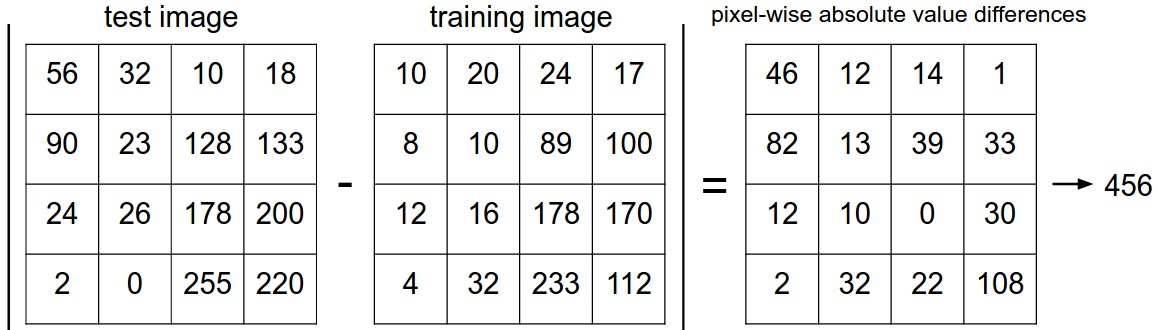
\includegraphics[scale=0.4]{images/l1distance.jpg}
Another approach for computing disatances between vectors is to use the \textbf{L2 distance}, which has the geometric interpretation of computing the euclidean distance between two vectors:
\begin{equation*}
    d_2(I_1,I_2) = \sqrt{\sum_{p}\left(I_1^p-I_2^p\right)^2}
\end{equation*}

\subsection{k-Nearest Neighbor Classifier}
The idea is very simple: finding the top \textbf{k} closest images, and have them vote on the label of the test image. In particular, when $k = 1$, it is the Nearest Neighbor Classifier. Intuitively, higher values of $k$ have a smoothing effect that makes the classifier more resistant to outlier, e.g. higher variance. In practice, you do not know what value of $k$ should you use? This leads to the next problem: \textbf{hyperparameter tuning}.

\paragraph{Validation sets for Hyperparameter tuning}
When working with many \textit{unknown} variables, we often call these various choices as \textbf{hyperparameters}. They come up very often in the design of many Machine Learning algorithms that learn from data, and it is often not obvious what values one should choose. We can attempt to use many different values; however, the key idea is \textbf{we cannot use the test set for the purpose of tweaking hyperparameters} because the algorithm would lose its generalization and bring higher variance, overfitting the test set. The usual way to deal with the problem is to use validation to tune these hyperparameters and verify them with the test data.

\paragraph{Cross-validation} the idea is that instead of arbitrarily picking the first 1000 datapoints to be the validation set and the rest as a training set, you can get better and less noisy estimate of how well a cretain value of $k$ works by iterating over different validation sets and averageing the performance across these. For example, in 5-fold cross validation, we should split the training into 5 equal folds, use 4 of them for training, and 1 for validation so that we can iterate over which fold is the validation fold, evaluate the performance, and finally average the performance across the different folds.

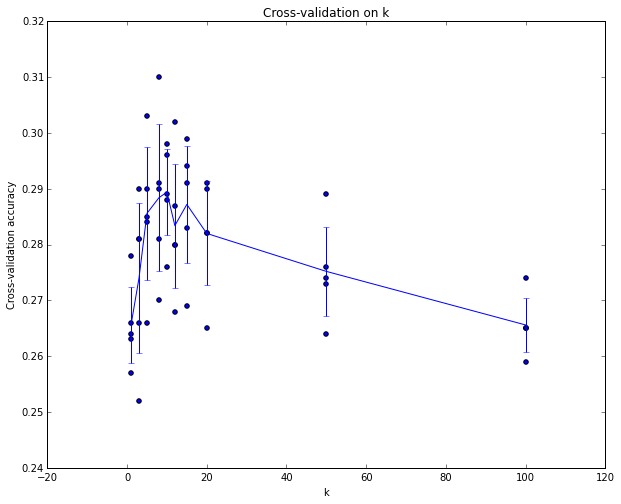
\includegraphics[scale=0.4]{images/cvplot.png} \\
From this plot, we can see that about $k = 7$ works best on this particular dataset (corresponding to the peak in the plot). If we used more than 5 folds, we might expect to see a smoother (i.e. less noisy) curve.

\subsection{Linear Classification}

\paragraph{Intro to Linear classification}
In the last section, we learn about k-Nearest Neighbor (kNN) classifier which labels images by comparing them to (annotated) images from the training set. As we saw, kNN has a number of disadvantages:
\begin{enumerate}
	\item The classfier must remember all of the training data, which causes a problem when the amount of data is large. \\
	\item Classifying a test image is expensive since it requires a comparison to all training images.
\end{enumerate}
Thus, we are now going to develop a more powerful approach to image classification that we'll eventually naturally extend to entire Neural Networks and Convolutional Neural Networks. This approach will have two major components: a \textbf{score function} that maps the raw data to class scores, and a \textbf{loss function} that quantifies the agreement between the predicted scores and the ground truth labels. We'll then cast this as an optimization problem in which we will minimize the loss function with respect to the parameters of the score function.

\paragraph{Linear score function}
Let's assume a training dataset of images $x_i \in \mathbb{R}^D$, each associated with a label $y_i$. Here $ i = 1,\ldots,N$ and $y_i \in {1,\ldots,K}$. That is, we have $N$ examples (each with a dimensionality $D$) and $K$ distinct categories. For examaple, in CIFAR-10 we have a training set of $N = 50000$ images, each with $D = 32 \times 32 \times 3 = 3072$ pixels, and $K = 10$, since there are 10 distinct classes. We will now define the score function $f: \mathbb{R}^D \rightarrow \mathbb{R}^K$ that maps the raw image pixels to class scores.
\subparagraph{Linear classifier}
We'll start out with arguably the simplest possible function, a linear mapping:
\begin{equation*}
	f(x_i,W,b) = Wx_i + b
\end{equation*}
In the above equation, we are assuming that the image $x_i$ has all of its pixels flattened out to a single column vector of shape $[D \times 1]$. The matrix $W$ (of size $[K \times D]$), and the vector $b$, usually called the \textbf{bias vector}, (of size $[K \times 1]$) are the \textbf{parameters} of the function. \\
It's important to note that we have control over the setting of the parameters \textbf{W, b}. Our goal is to set these in such a a way that the computed scores match the ground truth labels across the whole training set. Intuitively, we wish that the correct class has a score that is higher than the scores of incorrect classes. In addition, note that to classify the test image involves a single matrix multiplication and addition is signifcantly faster than to compare a test image to all training images.

\paragraph{Interpreting a linear classifier}
Notice that a linear classifier computes the score of a class as a weighted sum of all of its pixel values across all 3 of its color channels. Depending on precisely what values we set for these weights, the function has the capacity to like or dislike certain colors at certain positions in the image. For instance, you can imaging that the "ship" class might be more likely if there is a lot of blue on the sides of an image (which could correspond to water). \\
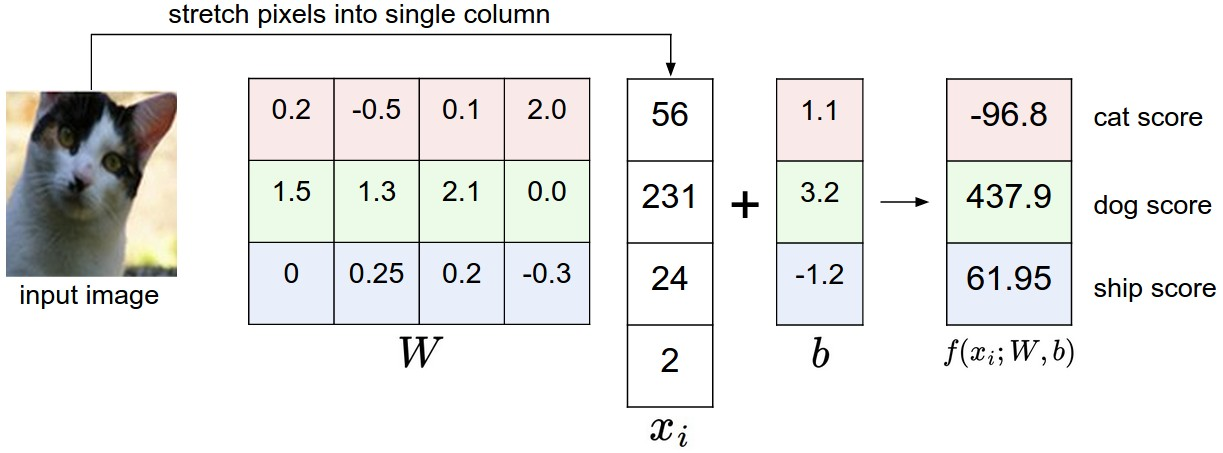
\includegraphics[scale=0.3]{images/imagemap.jpg} \\
Another interpretation for the weights $W$ is that each row of $W$ corresponds to a \textit{template} (or sometimes also called a \textit{prototype}) for one of the classes. The score of each class for an image is then obtained by comparing each template with the image using an inner product (or \textit{dot product}) one by one to find the one that "fits" best. Another way to think of it is that we are still effectively doing Nearest Neighbor, but instead of having thousands of training images we are only using a single image per class (although we will learn it, and it does not neccssarily have to be one of the images in the training set), and we use the (negative) inner product as the distance instead of the L1 or L2 distance.

\paragraph{Loss function}
In addition to have a function for measuring the score corresponding to each class, we also want to measure our unhappiness with outcomes so that it introduces a \textbf{loss function} (or sometimes also referred to as the \textbf{cost function} or the \textbf{objective}). Intuitively, the loss will be high if we're doing a poor job of classifying the training data, and it will be low if we're doing well.

\subsubsection{Multiclass SVM}
One of two most commonly used loss function is the \textbf{Multiclass Support Vector Machine} (SVM) loss, given that $f(x_i, W)$ is the scores for each class:
\begin{equation*}
	L = \frac{1}{N}\sum_{i}\sum_{j \ne y_i}\left[\max(0,f(x_i,W)_j - f(x_i,W)_{y_i} + \Delta)\right]
\end{equation*}
Visually, we want the loss function to differentiate the correct class from other incorrect classes by parameter $\Delta$ as shown in the figure below. \\
\begin{center}
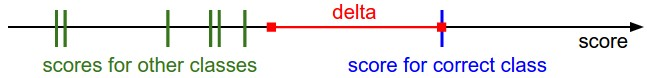
\includegraphics[scale=0.4]{images/margin.jpg}
\end{center}

\paragraph{Regularization} There is one minor bug with the loss function presented above. Suppose that we have a dataset and a set of parameteres $W$ that correctly classify evey example. The issue is that this set of $W$ is not necessarily unique: there might be many similar $W$ that correctly classify the examples as well. For instance, any multiply of these parameters, $\lambda W$, where $\lambda > 1$. This brings up to find a way to penalize the set of parameters that are not unique by favoring the parameters whose values are smaller. By using the \textbf{regularization penalty $R(W)$}, the \textit{loss function} will be changed to
\begin{equation*}
	L = \frac{1}{N}\sum_{i}\sum_{j \ne y_i}\left[\max(0,f(x_i,W)_j - f(x_i,W)_{y_i} + \Delta)\right] + \lambda \sum_k \sum_l W^2_{k,l}
\end{equation*}
where the latter term is \textbf{regularization loss}.

\subsubsection{Softmax classifier}
The other popular choice rather than SVM is the \textbf{Softmax classifier}, which has a different loss function that makes use of the logistic regression classifier. We replace the \textit{hinge loss} with a \textbf{cross-entropy loss} that has the form:
\begin{equation*}
	L_i = -\log\left(\frac{e^{f_{y_i}}}{\sum_j e^{f_j}}\right) \text{ \indent or equivalently \indent} L_i = -f_{y_i} + \log \sum_j e^{f_j}
\end{equation*}
where we are using the notation $f_j$ to mean the $j$-th element of the vector of class scores $f$. Oftentimes, $f_j(z) = \frac{e^{z_j}}{\sum_k e^{z_k}}$ is also called the \textbf{softmax function}: it takes a vector of arbitrary real-valued scores (in $z$) and squashes it to a vector of values between zero ans one that sum to one.

\paragraph{Practical issues: Numeric stability} When you're writing code for computing Softmax function in practice, the intermediate terms $e^{f_{y_i}}$ and $\sum_j e^{f_j}$ may vary very large due to the exponentials. Thus, dividing large numbers can be numerically unstable, so it is important to use a normalization trick. Notice that this expression is mathematically equivalent:
\begin{equation*}
	\frac{e^{f_{y_i}}}{\sum_j e^{f_j}} = \frac{Ce^{f_{y_i}}}{C\sum_j e^{f_j}} =
	\frac{e^{f_{y_i} + \log C}}{\sum_j e^{f_j + \log C}}
\end{equation*}
From the expression on the right, we can choose the value of $C$ that can solve the very large value of the exponentials. The simplest way is to set $\log C = -\max_j f_j$.

\subsubsection{SVM vs Softmax}
Basically, SVM will give a score corresponding to each class of the possible output; however, Softwax will give the "probabilities" that can give a sense of better thought of as confidences.
\begin{center}
	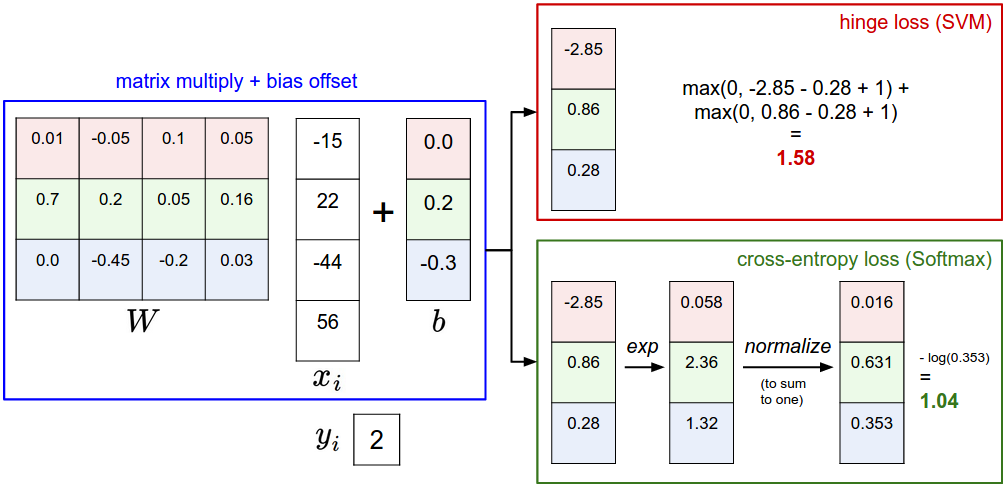
\includegraphics[scale=0.3]{images/svmvssoftmax.png}
\end{center}

\subsubsection{Optional: Deep Learning using Linear Support Vector Machines}
This paper is accessible on \url{http://arxiv.org/pdf/1306.0239v4.pdf}. \\
\indent This paper shows that simply changing the softmax activation function to linear SVMs gives significant gains on popular deep learning datasets MNIST, CIFAR-10, and the ICML 2013. \\
\indent Unlike the hinge loss of a standard SVM, the loss from the L2-SVM is differentiable and penalizes errors much heavily. From the study, they believe that the performance gain is largely due to the superior regularization effects of the SVM loss function, rather than an advantage from better parameter optimization.

\paragraph{Multiclass SVMs} We denote the output of the $k$-th SVM as
\begin{equation*}
	a_k(x) = w^Tx
\end{equation*}
and the predicted class is then
\begin{equation*}
	\arg \max_{k} a_k(x)
\end{equation*}

\paragraph{Deep Learning with Support Vector
Machines}
In this paper, they use L2-SVM to train deep deural nets for classification. Lower layer weights are learned by backpropagating the gradients from the top layer linear SVM. For the softmax classifier, we define the cost function, objective, as:
\begin{equation*}
	l(w) = \min_w \frac{1}{2}w^Tw + C\sum_{n=1}^{N}\max(1 - w^T x_n t_n,0)
\end{equation*}
Let the input $x$ replaced with the penultimate activation $h$,
\begin{equation*}
	\frac{\partial l(w)}{\partial h_n} = -Ct_n w\left(\mathbb{I}\{1 > w^Th_nt_n\}\right)
\end{equation*}
where $\mathbb{I{}}$ is the indicator function. Likewise, for the L2-SVM, we have
\begin{equation*}
	\frac{\partial l(w)}{\partial h_n} = -2Ct_n w\left(\max(1 - w^T h_n t_n, 0)\right)
\end{equation*}
From this point, we see that backpropagation algorithm is exactly the same as the standard softmax-based deep learning networks.

\paragraph{Experiment: Facial Expression Recognition} This challenged was hosted by the ICML 2013 workshop on representation learsning, organized by the LISA at University of Montreal. The data consist of 28,709 48x48 images of faces under 7 different types of expression. The winning solution, which succeed $69.4\%$ on the public validation and $71.2\%$ on the private test. This solution consists of using a simple Convolutional Neural Network with linear one-vs-all SVM at the top. Stochastic gradient descent with momentum is used for training and several models are averaged to slightly improve the generalization capabilities.  
\end{document}
